%!TEX root = ..\main.tex
%!TEX encoding = UTF-8 Unicode

%——————————————————————————————————————————————————————————
%	CHAPTER 4
%	translator: lh1962
%	proofreader: InSight, SI
%——————————————————————————————————————————————————————————
\newcommand\rd{\mathrm d}
\newcommand\ri{\mathrm i}

\chapter[框架/体系]{The Framework 框架/体系}\label{chap4}
这一章的基本思路是,我们要通过使{\it 某些东西}取极小值,得到正确的关于自然的方程。{\it 某些东西}是什么?有一件事是确定的:它不应该在 Lorentz 变换下改变,否则我们会在不同的参考系下得到不同的自然规律。在数学意义上,它意味着我们寻找的这个东西是个标量,依照 Lorentz 群的 \( (0,0) \) 表示作变换。再考虑到自然总依简单而行,我们已经足够导出关于自然的方程了。

从这个想法出发,我们将会引入{\bf 拉格朗日形式(Lagrangian formalism)}。通过使理论的中心对象取极小值,可以得到用以描述问题中的物理系统的运动方程。极小化过程的结果被称作 {\bf 欧拉-拉格朗日方程(Euler-Lagrange equations)}。

通过拉格朗日形式,可以得到物理中最重要的定理:{\bf Noether 定理( Noether’s Theorem)}。这个定理揭示了对称性和守恒量%
\mpar{守恒量指的是不随时间变化的物理量。例如一个给定体系的能量或动量。数学上意味着\(\rd Q/\rd t = 0 \rightarrow Q = \text{常数}\)。}%
之间的深刻联系。我们将在下一章中利用它来理解,理论是如何来描述实验测量量的。

\section[拉格朗日形式]{Lagrangian Formalism \quad 拉格朗日形式}\label{sec4.1}

拉格朗日形式是在基础物理中被广泛运用的一个强有力的框架%
\mpar{物理中当然有其他框架,例如以{\bf 哈密顿量(Hamiltonian)}为中心对象的{\bf 哈密顿形式(Hamiltonian formalism)}。哈密顿量的问题在于它不是洛伦兹不变的,因为它所代表的能量,仅仅是{\bf 协变能动矢量(covariant energy-impulse vector)}的一个分量}%
。由于理论的基本对象——{\bf 拉格朗日量(Lagrangian)}是一个标量%
\mpar{标量指依照洛伦兹群的 \( (0,0) \) 表示作变换的对象。这意味着它不在洛伦兹变换下改变}%
,它相对简单。如果你希望从对称性的观点考虑问题,这种形式将会是非常有用的。要求拉格朗日量的积分,{\bf 作用量(action)},在某些对称变换下不变,即保证了体系的动力学遵从该对称性。

\subsection{Fermat 原理}\label{sec4.1.1}
\begin{quote}
自然界中不论发生什么过程,由此造成作用量的改变总尽可能的小。


\begin{flushright}
- Pierre de Maupertius
\mpar{Recherche des loix du mouvement (1746)}
\end{flushright}
\end{quote}

拉格朗日形式的思想源于 Fermat 原理:光在两空间点间传播总依耗时最短的路径\(q(t)\)而行。数学上来讲,如果我们定义给定路径\(q(t)\)的作用量为
\[
S_{\text{light}}[{\mathbf q}(t)] = \int ~{\mathrm d}t
\]
而我们的任务便是找到一条特定的路径\(q(t)\)使作用量取极小值%
\mpar{此处的作用量仅仅是沿给定路径对时间的积分,但一般而言作用量会更加复杂,我们待会儿就能见到}%
为了得到一个给定{\bf 函数}的极小值%
\mpar{一般而言,我们希望找到{\bf 极值(extremums)},即极小值{\bf 和}极大值。下一节中的方法足以找到这两者。无论如何,我们将继续谈论极小值}%
,我们可以求得其导函数并令其为零;而为了找到{\bf 泛函}\(S[q(t)]\)——函数\(q(t)\)的函数\(S\)——的极小值,就得要一个新的数学工具:{\bf 变分法}。

\marginpar{
	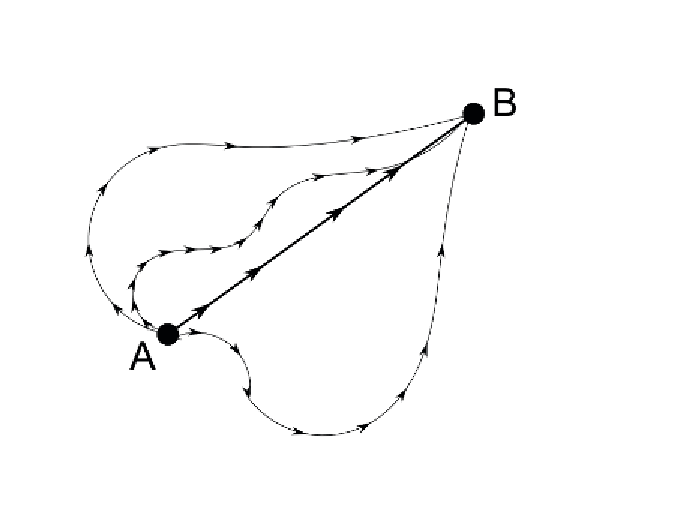
\includegraphics[scale=0.35]{./Figure/fig4_1}
	\figcaption{对于给定初末端点的路径的扰动}
}

\subsection{变分法:基本思想}\label{sec4.1.2}

在思考如何发展一套能够找到泛函极值的新理论之前,我们需要倒回去想想什么给出一个数学上的极小点。变分法给出的答案是,极小点由极小点邻域的性质决定。例如,让我们尝试寻找一个寻常函数\(f(x)=3x^2+x\)的极小点\(x_{\min}\)。我们从一个特定点\(x=a\)出发,仔细考察其邻域。数学上它意味着\(a + \epsilon\),其中\(\epsilon\)代表无穷小量(可正可负)。我们将\(a\)的变分代入函数\(f(x)\):
\[
f(a+\epsilon) = 3(a+\epsilon)^2+(a+\epsilon) = 3(a^2+2a\epsilon+\epsilon^2)+a+\epsilon \text{。}
\]
如果\(a\)是极小点,\(\epsilon\)的一阶变分必须为零,否则我们可以取\(\epsilon\)为负\(\epsilon < 0\),这样\(f(a+\epsilon)\)就会比\(f(a)\)更小%
\footnote{\textcolor{red}{译注:此处讨论有误。可改作“否则若$\epsilon$的一阶变分为正,我们可以\dots ,反之亦然。”}}%
。因此,我们将线性依赖于\(\epsilon\)的项取出并令其为零。
\[
3 \cdot 2a\epsilon + \epsilon \overset{\text{!}}{=} 0 \rightarrow 6a+1\overset{\text{!}}{=}0\text{。}
\]
由此我们找到极小点
\[
x_{\min} = a = -\frac{1}{6} \text{,}
\]
它自然和我们求导\(f(x)=3x^2+x\rightarrow f'(x)=6x+1\)并令其为零的办法得到的结果一致。对于寻常函数而言,这只是一个用来干同一件事不同方法而已%
\footnote{译注:对于受微元法茶毒的物竞生而言,求导才是用来干这件事的不同方法。}%
,但是变分法却能找到泛函的极值点。我们马上就能看到,应当如何处理一个一般的作用量泛函。

拉格朗日形式的中心思想在于,对于有质量的物体也存在一个与光的 Fermat 原理相类似的原理。当然,它不可能直接遵从费马原理,但是我们可以从一个更一般的形式出发
\[
S[q(t)]=\int {\mathcal L}~{\mathrm d}t
\]
其中\(\mathcal L\)一般是一个非常数的参量,称为拉格朗日量。对于光而言,这个参量是个常数。一般的,拉格朗日量依赖于物体的坐标和速度\({\mathcal L}={\mathcal L}(q(t),\frac{\partial}{\partial t} q(t))\)。下一节中我们将仔细讨论这件事%
\mpar{我们的任务是找到对于给定拉格朗日量和初始条件有着最小作用量的路径\(q(t)\)。在此之前,我们得先找到正确的拉格朗日量,用以描述问题中的物理系统。这是我们在上一章中所讨论的对称性所能发挥作用的地方。通过要求拉格朗日量在洛伦兹群的所有变换下不变,我们就能找到正确的拉格朗日量}%
。在仔细讨论如何对这样一个泛函使用变分法之前,我们需要先讲讲两个小问题。

\section[限制]{Restrictions \quad 限制}\label{sec4.2}
正如\ref{sec1.1}节所提到的,现有理论中有些限制条件无法从第一性原理中得到。我们所能知道是,如果想得到一个有意义的理论,我们必须加上这些限制。

一个重要的限制是,我们仅允许拉格朗日量中出现尽可能低阶的非平凡%
\footnote{译注:Non-trival. Trival 这个词常包含简单、弱智、无意义之义。}%
导数。这里平凡指的是对于系统的动力学,即运动方程,没有影响。某些理论会包含一阶导数,另外一些带二阶导数。一个给定理论所含的最低阶导数由该条件决定:拉格朗日量在 Lorentz 变换下不变%
\mpar{实际上,作用量才应该是 Lorentz 不变的。但如果拉格朗日量满足这个条件,那作用量自然也是。}%
,否则我们将在不同的参考系下导出不同的运动方程%
\footnote{\textcolor{red}{译注:此处讨论疑有误,作者此前并没有说明积分中的时间是坐标时还是固有时}}%
。对于某些理论,我们无法写出一个仅含一阶导数项的不变量,那么此时二阶导数便成了最低阶导数项。

我们并不清楚如何处理包含高阶导数的理论,它们有一些根本的困难%
\mpar{这些困难称为 Ostrogradski 不稳定性,即包含高阶导数的系统的能量没有下界,以至于系统中的所有态总会自发衰变到能量更低的态上去。这类系统中找不到稳定的状态。}%
。另外,拉格朗日量中的高阶导数会使得运动方程中也包含高阶导数,这样就必须知道更多的初始条件才能决定物体的运动。

有些人会宣称对理论所包含导数阶数的限制源于我们希望得到一个局域%
\mpar{局域性是狭义相对论的基本假定,\ref{sec2.4}已作阐述}%
理论,但这个要求仅会排除掉那些无穷阶导数。一个非局域相互作用有如下形式%
\mpar{我们将会讨论粒子的拉格朗日理论:寻求粒子的路径;也会讨论场的拉格朗日理论:寻求场函数\(\Phi(x)\)。这将是下一节的主题。}
\begin{equation}
\Phi(x-h)\Phi(x)
\end{equation}
即,时空中距离为\(h\)的两个点的场相互作用。利用 Taylor 展开我们有%
\footnote{\textcolor{red}{译注:此式有误,已更正}}
\begin{equation}
\Phi(x-h) = \sum\limits_{k=0}^{\infty}\left(\left(\frac{\partial}{\partial x}\right)^k\left.\Phi(x)\right|_{x}\right) \frac{(-h)^k}{k!}
\end{equation}
即包含无穷阶导数会导致一个非局域的理论。

另外一个限制是,要得到一个自由(无相互作用)场/粒子的理论,我们只能写到二次项。这意味着我们只会考虑%
\mpar{从另外一个角度来看,这再次表示我们只引入最低阶的非平凡项。我们随后就会看到,含\(\Phi^0\)和\(\Phi^1\)的项是平凡的,因此我们这次用的是\(\Phi\)的最低阶非平凡项}
\[
\Phi^0, \Phi^1, \Phi^2
\]
这样的项。例如,形如\(\Phi^2 \partial_\mu \Phi\)的项是\(\Phi\)的三阶项,因而不会被包含在我们自由理论的拉格朗日量中。

\section[粒子理论与场论]{Particle Theories vs. Field Theories \quad 粒子理论与场论}\label{sec4.3}
我们目前有两套用以描述自然的理论框架。一套是粒子理论,用依赖于时间的粒子位置描述物理系统,即\(\vec{q}=\vec{q}(t)\)。由于我们不是非得在使用笛卡尔坐标系%
\mpar{例如,我们可以用球坐标系}%
,所以用的是字母\(q\)而不是\(x\)。对于这样的理论,拉格朗日量依赖于坐标\(\vec{q}\),速度\(\partial_t\vec{q}\)和时间\(t\):%
\footnote{译注:严格说来,依赖于坐标函数\(\vec{q}(t)\),速度函数\(\partial_t\vec{q}(t)\)和时间\(t\)}
\begin{equation}
{\mathcal L} = {\mathcal L} (\vec{q},\partial_t\vec{q},t)
\end{equation}

一个著名的拉格朗日量是\({\mathcal L} = \frac{1}{2}m\vec{q}^2\),它能导出经典力学中的 Newton 运动方程。在稍后将进行相当详细的讨论。

另一套是场论:使用场而不是独立粒子的坐标来描述自然%
\mpar{量子场论有一个特别优美的性质是关于如何将粒子引进的。我们将在\ref{chap6}中看到场有能力产生和湮灭粒子}%
。在这套理论中,时空构成了场\(\Phi(\vec{x},t)\)表演的舞台。利用前面提到过的限制,我们得到%
\mpar{这里我故意使用了不同的符号\({\mathscr L}\),因为在场论中大多数时候我们都在和拉格朗日量密度\({\mathscr L}\)打交道。两者之间满足关系式\({\mathcal L} = \int{\mathrm d}^3\bm{x}~{\mathscr L}\)}
\begin{equation}
{\mathscr L} = {\mathscr L} (\Phi(\vec{x},t), \partial_\mu \Phi(\vec{x},t), \vec{x})
\end{equation}

这里一个著名的拉格朗日量密度\({\mathscr L} = \frac{1}{2}\left(\partial_\mu\Phi\partial^\mu\Phi-m^2\Phi^2\right)\),它可以导出 Klein-Gordon 方程。

场论的一大优点是它将时空等价的对待。在粒子理论中我们使用空间坐标\(\vec{q}(t)\)作为时间的函数来描述粒子。尤其是,拉格朗日量中没有类似于\(\partial_{\vec{q}}t\)的项(如果出现了这类项,我们该怎样理解它呢?)当我们讨论粒子的坐标时,意义是清楚的,但对时间做类似的陈述时,却很难有明确的意义%
\footnote{译注:利用不那么古老的相对论性语言,粒子理论下时空坐标是可以在形式上被同等对待的:用以求导的东西只能是曲线的参数,它可以取作粒子世界线的固有时、某一坐标系的坐标时、或者其他什么东西(只要性质合适,也可以是空间坐标);而时空坐标则被同样的求导。}。

讨论了这么多,我们终于可以回到这章开头所说的极小化问题上来了。我们希望找到某些泛函
\[
S[q(t)] = \int {\mathcal L}~{\mathrm d}t
\]
的极小值,以得到正确的运动方程。

对于粒子而言,方程的解是使得泛函取极小值的正确路径;而对于场而言,解是正确的场函数。

此刻请不用担心\(\mathcal L\)的具体形式,下面数章将详细讨论如何对问题中的系统导出正确的拉格朗日量\({\mathcal L}\)。现在,我们将使用之前所介绍过的变分法,对于一个一般的\(\mathcal L\)导出泛函\(S[q(t)]\)的极小值。极小化过程将给出系统的运动方程。

\section[欧拉-拉格朗日方程]{Euler-Lagrange equation \quad 欧拉-拉格朗日方程}\label{sec4.4}
我们从粒子理论出发,它能让我们搞清楚,在给定初末端点后,粒子是如何在两点间运动的。数学上,即寻找{\bf 函数}\(q(t)\)使得作用量\footnote{译注:此处原文字体有误,已更正}
\[
S = \int_{t_1}^{t_2} {\mathcal L}\left(q(t),\frac{\rd q(t)}{\rd t},t\right)
\]
取极值(极大值或极小值)。

使用记号
\[
\dot q(t) = \frac{\rd q(t)}{\rd t}\text{。}
\]
与之前的例子类似,取\(q(t)=a(t)\)并让对这个函数进行一个扰动
\[
a(t) + \epsilon(t)
\]
其中\(\epsilon\)依旧是一个无穷小量。对于一个粒子而言,我们必须同时改变其速度\(\dot a(t) + \dot\epsilon(t)\),其中\(\dot\epsilon(t) = \frac{\rd \epsilon(t)}{\rd t}\)。

在边界上,扰动后的路径应与原路径相同:
\begin{equation}
0 = \epsilon(t_1) = \epsilon(t_2)
\label{equ4.5}
\end{equation}
这是因为我们寻找的是使作用量积分取极值的{\bf 给定初末端点}的路径。

这个扰动使得泛函变为
\[
S = \int_{t_1}^{t_2} {\mathcal L}\left(q+\epsilon,\dot q + \dot \epsilon, t\right)~\rd t \text{。}
\]
与之前的例子类似,极小值要求线性依赖于扰动\(\epsilon\)的项为零。由于我们处理的是一般的\(\mathcal L\),故将其展开成 Taylor 级数%
\mpar{我们使用的是这个公式的多变量形式,参见附录\ref{appendix.B.3}:
\[
\begin{aligned}
{\mathcal L}\left(q+\epsilon,\dot q + \dot \epsilon, t\right) = {\mathcal L}(q,\dot q,t) + \\
\epsilon\frac{\partial \mathcal{L}}{\partial q} + \dot\epsilon\frac{\partial \mathcal{L}}{\partial \dot q} + \dots
\end{aligned}
\]}%对原文公式有改动
,并令一阶项为零
\begin{equation}
\int_{t_1}^{t_2} \rd t ~ \left[ \epsilon(t) \frac{\partial \mathcal{L}}{\partial q} + \left( \frac{\rd}{\rd t} \epsilon(t) \right)\frac{\partial \mathcal{L}}{\partial \dot q} \right] \overset{\text{!}}{=} 0 \text{。}
\label{equ4.6}
\end{equation}
对后一项做分部积分%
\mpar{分部积分是莱布尼兹律的直接推论,详见附录\ref{appendix.B.2}}%
得到
\[
\begin{aligned}
\int_{t_1}^{t_2} \rd t ~ \left( \frac{\rd}{\rd t} \epsilon(t) \right)\frac{\partial \mathcal{L}(q,\dot q,t)}{\partial \dot q} =\\
\left.\epsilon(t)\frac{\partial \mathcal{L}(q,\dot q,t)}{\partial \dot q}\right|_{t_1}^{t_2} - \int_{t_1}^{t_2} \rd t ~  \epsilon(t) \frac{\rd}{\rd t} \left( \frac{\partial \mathcal{L}(q,\dot q,t)}{\partial \dot q} \right)
\end{aligned}
\]
利用\ref{equ4.5}式有
\[
\left.\epsilon(t)\frac{\partial \mathcal{L}(q,\dot q,t)}{\partial \dot q}\right|_{t_1}^{t_2} = 0
\]
因此,我们可以将\ref{equ4.6}改写为
\[
\int_{t_1}^{t_2} \rd t ~\epsilon(t) \left[ \frac{\partial \mathcal{L}}{\partial q} - \frac{\rd}{\rd t} \left( \frac{\partial \mathcal{L}(q,\dot q,t)}{\partial \dot q}\right) \right] \overset{\text{!}}{=} 0
\]
易见上式对于任意扰动\(\epsilon(t)\)为零仅当方括号\([~]\)内的表达式为零。故有%
\mpar{可能你会对于两类不同的导数符号感到困惑。\(\frac{\rd}{\rd t}\)被称作对\(t\)的全导数,而\(\frac{\partial}{\partial t}\)被称为偏导数。全导数给出总改变量,函数\(f\)的变化率,即偏导数,乘以变量自身的改变,之和。
例如,三维空间中的函数\(f(x(t),y(t),z(t))\)的总变化率为\(\frac{\rd f}{\rd t} = \frac{\partial f}{\partial x}\frac{\partial x}{\partial t}+\frac{\partial f}{\partial y}\frac{\partial y}{\partial t}+\frac{\partial f}{\partial z}\frac{\partial z}{\partial t}\)。
即变化率乘以自身的改变量。
相对的,偏导数仅给出总改变量的一部分。对于一个不显式的依赖于\(t\)的函数,其偏导数为零。例如,对于\(f(x(t),y(t))=x^2y+y^3\),我们有\(\frac{\partial f}{\partial t}=0\),但\(\frac{\partial f}{\partial x}=2xy \ne 0, \frac{\partial f}{\partial y}=x^2+3y^2 \ne 0\)。
因此\(\frac{\rd f}{\rd t}=2xy\frac{\partial x}{\partial t}+(x^2+3y^2)\frac{\partial y}{\partial t}\)。
作为对比,对于另一个函数\(g(x(t),y(t),t)=x^2t+y\)我们有\(\frac{\partial g}{\partial t}=x^2\)
}
\begin{equation}
\frac{\partial \mathcal{L}}{\partial q} - \frac{\rd}{\rd t} \left( \frac{\partial \mathcal{L}(q,\dot q,t)}{\partial \dot q} \right)= 0
\label{equ4.7}
\end{equation}
这就是著名的{\bf 欧拉-拉格朗日方程(Euler-Lagrange equation)}

我们可以用类似的办法处理场论。首先,注意到场论将时空同等对待。因此引入拉格朗日量密度:
\begin{equation}
{\mathcal L} = \int{\mathrm d}^3\bm{x}~{\mathscr L}(\Phi^i,\partial_\mu \Phi^i)
\end{equation}
并用拉格朗日量密度来表示作用量
\begin{equation}
S = \int \rd t~{\mathcal L} = \int{\mathrm d}^4\bm{x}~{\mathscr L}(\Phi^i,\partial_\mu \Phi^i)
\end{equation}
依照上面讲过的步骤,我们可以得到场的运动方程组%
\mpar{在这里用“组”字是因为对于每一个场分量\(\Phi_1,\Phi_2,\dots\)我们都可以得到一个方程}%
:
\begin{equation}
\frac{\partial \mathscr{L}}{\partial \Phi} - \partial_\mu \left( \frac{\partial \mathscr{L}}{\partial (\partial_\mu \Phi)} \right)= 0
\label{equ4.10}
\end{equation}

下一节中将在拉格朗日形式下导出近代物理学中重要的一个定理。从中可以看到对称性与守恒量之间的深刻联系。守恒量是描述自然的合适参量%
\mpar{我们将其视做锚定这个复杂的世界之物。不论万事万物如何改变,守恒量依旧是守恒量。}%
,这个定理将教会我们如何和它打交道。

\section[Noether 定理]{Noether's Theorem \quad Noether 定理}\label{sec4.5}
Noether 定理表示,拉格朗日量的每一个对称性都直接对应一个守恒量。换言之,物理学家用于描述自然(守恒量)的记号和对称性直接相关。这确实是科学史上最美的创见之一。

\subsection{粒子理论的Noether 定理}\label{sec4.5.1}
先看看能对粒子理论中的守恒量做点什么。我们限于讨论连续对称性,这样才能使用无穷小变换。如同上一章所言,重复进行无穷小变换可以得到一个有限变换。拉格朗日量在无穷小变换%
\mpar{用符号\(\delta\)来表述小扰动,希望不会和用来表述偏导数的\(\partial\)相混淆。}%
\(q\rightarrow q'=q+\delta q\)下不变的性质用数学表述如下%
\footnote{译者注:该书中$\delta S$,$\delta {\mathcal L}$与平常的约定都差了一个负号。}
\begin{equation}
\begin{aligned}
\delta {\mathcal L} &= {\mathcal L}(q,\frac{\rd q}{\rd t},t) - {\mathcal L}(q+\delta q,\frac{\rd (q+\delta q)}{\rd t},t) \\
&= {\mathcal L}(q,\frac{\rd q}{\rd t},t) - {\mathcal L}(q+\delta q,\frac{\rd q}{\rd t}+\frac{\rd \delta q}{\rd t},t) \overset{\text{!}}{=} 0
\end{aligned}
\label{equ4.11}
\end{equation}

要求拉格朗日量是变换不变的,这个限制太强了。为了保证动力学一样,不变的应该是作用量而不是拉格朗日量。当然,如果拉格朗日量不变,作用量自然不变:
\begin{equation}
\delta S = \int \rd t~{\mathcal L}(q,\frac{\rd q}{\rd t},t) -  \int \rd t~{\mathcal L}(q+\delta q,\frac{\rd q}{\rd t},t) = \int \rd t~\delta{\mathcal L}\underbrace{=}_{\mathclap{\text{若}~\delta{\mathcal L}=0}} 0
\end{equation}
在什么情况下,拉格朗日量改变而作用量不变呢?答案是,给拉格朗日量加上一个任意函数$G$对时间的全导数
\[
{\mathcal L}\rightarrow{\mathcal L}+\frac{\rd G}{\rd t}
\]
这时作用量不变%
\mpar{用到了$\delta G =\frac{\partial G}{\partial q}\delta q$。这是因为$G=G(q)$而我们改变了$q$,故$G$的扰动等于改变率$\frac{\partial G}{\partial q}$乘上$q$的扰动}
\[
\delta S \rightarrow \delta S' = \delta S + \int_{t_1}^{t_2} {\rd t~\frac{\rd}{\rd t}\delta G} = \delta S + \underbrace{\left.\frac{\partial G}{\partial q} \delta q \right|_{t_1}^{t_2}}_{\mathclap{=0~\text{因为}~\delta q(t_1)=\delta q(t_2)=0}}.
\]
最后一步中用到了扰动$\delta q$在初末时刻\footnote{译注:右侧删去了原文的一对括号}$t_1,t_2$为零。由此可知,拉格朗日量的扰动$\delta {\mathcal L}$不必非要为零,而仅需满足一个更弱的条件
\begin{equation}
\delta {\mathcal L} \overset{\text{!}}{=} \frac{\rd G}{\rd t}\text{。}
\label{equ4.13}
\end{equation}

这意味着拉格朗日量可以在不改变作用量和运动方程的情况下,加减某个函数的全微分$\frac{\rd G}{\rd t}$。将\ref{equ4.11}式的右端由$0$改作$\frac{\rd G}{\rd t}$,我们有
\begin{equation}
\delta {\mathcal L} =  {\mathcal L}(q,\frac{\rd q}{\rd t},t) - {\mathcal L}(q+\delta q,\frac{\rd q}{\rd t}+\frac{\rd (\delta q)}{\rd t},t) \overset{\text{!}}{=} \frac{\rd G}{\rd t}
\end{equation}
将第二项按 Taylor 级数展开到$\delta q$的一阶项,并使用记号$\frac{\rd q}{\rd t}=\dot q$
\begin{equation}
\begin{aligned}
&\rightarrow \delta {\mathcal L} =  {\mathcal L} - {\mathcal L} -\frac{\partial \mathcal L}{\partial q} \delta q - \frac{\partial \mathcal L}{\partial \dot q} \delta \dot q \overset{\text{!}}{=} \frac{\rd G}{\rd t}  \\
&\rightarrow \delta {\mathcal L} =  -\frac{\partial \mathcal L}{\partial q} \delta q - \frac{\partial \mathcal L}{\partial \dot q} \delta \dot q \overset{\text{!}}{=} \frac{\rd G}{\rd t}
\end{aligned}
\label{equ4.15}
\end{equation}
利用欧拉-拉格朗日方程\mpar{\ref{equ4.7}式:$\frac{\partial \mathcal L}{\partial q} = \frac{\rd}{\rd t} \left(\frac{\partial \mathcal L}{\partial \dot q}\right)$}重写\ref{equ4.15}式,有
\[
\rightarrow \delta {\mathcal L} =  -\frac{\rd}{\rd t} \left(\frac{\partial \mathcal L}{\partial \dot q}\right) \delta q - \frac{\partial \mathcal L}{\partial \dot q} \delta \dot q \overset{\text{!}}{=} \frac{\rd G}{\rd t}
\]
利用莱布尼兹律\mpar{如果你对莱布尼兹律仍有疑问,请参考\ref{appendix.B.1}},我们有
\begin{equation}
\begin{aligned}
&\rightarrow \delta {\mathcal L} =  -\frac{\rd}{\rd t} \left(\frac{\partial \mathcal L}{\partial \dot q}\delta q\right) \overset{\text{!}}{=} \frac{\rd G}{\rd t} \\
&\rightarrow\frac{\rd}{\rd t} \underbrace{\left(\frac{\partial \mathcal L}{\partial \dot q}\delta q + G\right)}_{\equiv J} \overset{\text{!}}{=} 0
\end{aligned}
\label{equ4.16}
\end{equation}
由此得到了一个不随时间变化的物理量$J$:
\begin{equation}
J = \frac{\partial \mathcal L}{\partial \dot q}\delta q + G\text{,}
\end{equation}
这是因为
\[
\frac{\rd J}{\rd t} = 0 \rightarrow J = \text{常数。}
\]

为了看清楚这一点,先借用一下后面章节的结论:常质量自由粒子的 Newton 第二定律是%
\mpar{如果$q$代表某个物体的位置,则$\frac{\rd q}{\rd t}=\dot q$是这个物体的速度,$\frac{\rd}{\rd t}\frac{\rd q}{\rd t}=\frac{\rd^2 q}{\rd t^2}=\ddot q$是加速度。}
\begin{equation}
m{\ddot\vec{q}} = 0 \text{。}
\end{equation}
相应的拉格朗日量是%
\mpar{我们现在处理的是高于一维的问题,所以使用矢量$\vec q$和$\vec a$而不是$q$和$a$。}
\begin{equation}
{\mathcal L}=\frac{1}{2}m\dot\vec{q}^2
\end{equation}
你可以将其代入欧拉-拉格朗日方程(\ref{equ4.7}式)中去验证它。

让我们从这个拉格朗日量出发,计算不同对称性所分别对应的守恒量。

由于${\mathcal L}=\frac{1}{2}m{\dot\vec q}^2$不依赖于$\vec q$,故此拉格朗日量在空间平移变换$\vec{q}\rightarrow\vec{q}+\vec{a}$不变($\delta{\mathcal L}=0$)。这个对应的守恒量满足条件\ref{equ4.13},即$G=0$的情形\footnote{译注:求和约定,见第\ref{chap3}章边注129}
\begin{equation}
J_\text{trans} = \frac{\partial\mathcal L}{\partial \dot\vec q} \vec a = m {\dot\vec q} {\vec a} = \vec{p}\vec{a} \text{,}
\end{equation}
其中$\vec{p}=m{\dot\vec q}$是经典力学中的{\bf 动量(momentum)}。由于等式$\frac{\rd J}{\rd t}$对于任意$\vec a$都成立,所以说:{\bf 拉格朗日量的空间平移不变性导致了动量守恒。}

现在考虑旋转变换,这得需要大于一的维度,因为一维上的旋转是没有意义的。下面将不会使用类似$\vec q$的矢量符号,而是更方便的指标记号。我们能将所有方程简单的用$\vec{q}\rightarrow q_i$改写。考虑无穷小旋转%
\mpar{这里我们用 Levi-Civita 符号来写旋转生成元。参见\ref{equ3.63}式下的文字。}%
$q_i \rightarrow q_i + \epsilon_{ijk} q_j a_k$,由此$\delta q_i=\epsilon_{ijk}q_j a_k$。仍然是因为由于${\mathcal L}=\frac{1}{2}m{\dot\vec q}^2$不依赖于$\vec q$,我们的拉格朗日量在这样的变换下也不改变,其对应的守恒量是%
\mpar{下式由\ref{equ4.16}式导出,这里对应的依旧是$G=0$的情况}
\begin{equation}
\begin{aligned}
J_\text{rot} =& \frac{\partial {\mathcal L}(q_i, \dot q_i, t)}{\partial \dot q_i}\delta q_i  = \frac{\partial \mathcal L}{\partial \dot q_i} \epsilon_{ijk} q_j a_k \\
  =& m {\dot q_i} \epsilon_{ijk} q_j a_k = m p_i\epsilon_{ijk} q_j a_k \\
  \rightarrow J_\text{rot} =& (\vec{p}\times\vec{q})\cdot\vec{a} \equiv \vec{L}\cdot\vec{a}
\end{aligned}
\end{equation}
在最后一步中我们将表达式用矢量记号重新写出,其中$\times$称作叉乘,而$\vec L$是经典力学中{\bf 角动量(angular momentum)}。即:{\bf 旋转不变性导致了角动量守恒。}

接下来让我们看看时间平移不变性%
\mpar{这意味着物理不会管我们是在昨天、今天还是五十年后做的实验,给定相同的初始条件,物理定律不会变化。}%
。一个无穷小的时间平移$t\rightarrow t'=t+\epsilon$会导致
\begin{equation}
\begin{aligned}
\delta {\mathcal L} &= {\mathcal L}\left(q(t),\frac{\rd q(t)}{\rd t},t\right) - {\mathcal L}\left(q(t+\epsilon),\frac{\rd q(t+\epsilon)}{\rd t},t+\epsilon\right) \\
&= -\frac{\partial \mathcal L}{\partial q}\frac{\partial q}{\partial t}\epsilon -\frac{\partial \mathcal L}{\partial\dot q}\frac{\partial\dot q}{\partial t}\epsilon -\frac{\partial\mathcal L}{\partial t}\epsilon \underbrace{=}_{\mathclap{\text{等式左端正好为全导数}}} -\frac{\rd \mathcal L}{\rd t}\epsilon \text{,}
\end{aligned}
\end{equation}
这表明一般而言$\delta{\mathcal L} \ne 0$,但有$G=-{\mathcal L}$。

将其代入\ref{equ4.16}式,有\footnote{译注:原文有字体混乱,已更正}
\begin{equation}
\frac{\rd}{\rd t}\underbrace{\left(\frac{\partial\mathcal L}{\partial\dot q}\dot q-{\mathcal L}\right)}_{\equiv\mathcal H} = 0
\end{equation}
守恒量$\mathcal H$称为{\bf 哈密顿量(Hamiltonian)},代表了系统的总能量。对于这个例子,我们有
\begin{equation}
\begin{aligned}
\mathcal H =& \frac{\partial\mathcal L}{\partial\dot q}\dot q-{\mathcal L} = \underbrace{\left(\frac{\partial}{\partial\dot q}\frac{1}{2}m{\dot q}^2\right)}_{\mathclap{=m{\dot q}}}\dot q - \frac{1}{2}m{\dot q}^2 \\
 =& m{\dot q}^2 - \frac{1}{2}m{\dot q}^2 = \frac{1}{2}m{\dot q}^2 \text{,}
\end{aligned}
\end{equation}
正好是系统的动能。由于这里没有势场或外力,故动能就是总能量。能导出在外势场中运动的粒子的 Newton 第二定律$m\ddot q=-\frac{\partial V}{\partial q}$\footnote{\textcolor{red}{原文有误,已更正}}的拉格朗日量是
\[
{\mathcal L} = \frac{1}{2}m{\dot q}^2 - V(q)\text{。}
\]
其哈密顿量为
\[
{\mathcal H} = \frac{1}{2}m{\dot q}^2 + V
\]
的确是正确的总能量(等于动能加势能)。

由{\bf 推动不变性(boost invariance)}导致的守恒量略有些奇怪,相应的计算放在了这一章的附录\ref{sec4.6}中。其结果为
\begin{equation}
\tilde{J}_\text{boost} = \underbrace{pt-\frac{1}{2}mvt}_{\mathclap{\equiv \tilde{p}t}}-mq=\tilde{p}t-mq
\end{equation}
我们可以看到这个量依赖于时间零点,可以通过恰当的选取时间零点使其为零。由于这个量是守恒量,这个守恒律告诉我们零始终都是零。\footnote{译注:这个守恒率没有说的那么平庸,事实上,它等价于质心运动定理;\textcolor{red}{又注:该结果以及\ref{sec4.6}的推导有误,参见译注\hyperref[note:boost]{21}}}

作为粒子理论的总结,我们得到了如下关系:
\begin{itemize}
\item 空间平移不变性$\Rightarrow$动量守恒
\item 推动不变性\mpar{推动的另一个叫法是动量空间的平移,因为变换$q\rightarrow q+vt$使动量$m\dot q\rightarrow m(\dot q+v)$}$\Rightarrow~\tilde{p}t-mq$守恒
\item 旋转不变性$\Rightarrow$角动量守恒
\item 时间平移不变性$\Rightarrow$能量守恒
\end{itemize}
Noether 定理向我们展示了,为什么这些记号%
\mpar{除了推动不变性导致的守恒量}%
会以这个或那个形式出现在形形色色的物理理论中。只要我们依旧有通常的时空对称性,动量、能量和角动量就是守恒量。在场论中,有两类对称性:一方面,拉格朗日量会在时空变换(如旋转)下不变;另一方面,我们也会有在场自身的变换下的不变性,称为{\bf 内禀对称性(internal symmetries)。}

\subsection{场论中的 Neother 定理——时空对称性}\label{sec4.5.2}
对于场,我们得区分在时空变换下两类不同的改变。当观测者$S$看到场$\Psi(x)$时,观测者$S'$看到的则是场$\Psi'(x')$。这是同一个场,只是从不同的视角来看,会有不同的分量值。这两类描述之间由 Lorentz 群中的一个合适的变换相联系。我们现在将会使用在\ref{sec3.7.11}中介绍过的场表示%the field representation
。(无穷维)微分算符表示$x$变换到$x'$。这意味着利用这个表示我们能在不同的时空点或者在一个旋转参考系中计算场分量。Lorentz 群的有限维变换使$\Psi$映射到$\Psi'$,即,混合场分量%
\mpar{请回忆这个例子,Weyl 旋量有两个分量而矢量场有四个分量。如果我们从一个不同的视角来考察矢量场$A_\mu=\begin{pmatrix} A_0\\ A_1\\ A_2\\ A_3 \end{pmatrix}$,即,从旋转系看,它会形如$A'_\mu=\begin{pmatrix} A'_0\\ A'_1\\ A'_2\\ A'_3 \end{pmatrix}=\begin{pmatrix} A_0\\ -A_2\\ A_1\\ A_3 \end{pmatrix}$。$A'_\mu$和$A_\mu$描述了从两个相差了绕$z$轴旋转$\unit{90}{\degree}$的坐标系分别观察到的同一个场。}。

对于一个依赖于时空的场的具体变换,需要同时考虑两个部分。我们将分别处理它们,首先来看$x$到$x'$的这一项。对于旋转来说,单由这一个部分推出的守恒量并不会真的守恒,这是因为我们忽略了变换的第二项。仅当将变换的两项$x\rightarrow x'$和$\Psi\rightarrow\Psi'$分别导致的守恒量加起来之后得到的,才是真正守恒的。

为了使上面这段论证更有说服力,我们考虑一个一般的拉格朗日量密度${\mathscr L}\left(\Phi(x_\mu),\partial_\mu \Phi(x_\mu),x_\mu\right)$\footnote{译注:原文多出一左括号}。对称性意味着
\begin{equation}
{\mathscr L}\left(\Phi(x_\mu),\partial_\mu \Phi(x_\mu),x_\mu\right) = {\mathscr L}\left(\Phi'(x'_\mu),\partial_\mu \Phi'(x'_\mu),x'_\mu\right)\text{。}
\end{equation}
一般的,当函数自身发生改变且其计算的点也发生改变时,函数的函数的总改变量由下式给出%
\mpar{如果你对此不熟悉:这常被称为全导数。总改变量等于变化率,即偏导数,乘以变量自身的改变,之和。例如,三维空间中的函数\(f(x,y,z)\)的总该变量为\(\frac{\partial f}{\partial x}\delta x+\frac{\partial f}{\partial y}\delta y+\frac{\partial f}{\partial z}\delta z\),即变化率乘以自身改变的距离。我们考察的是无穷小变化,故我们可以略去 Taylor 展开的高阶项仅考虑第一项。}
\begin{equation}
\delta f(g(x),h(x),\dots)=\frac{\partial f}{\partial g}\delta g + \frac{\partial f}{\partial h}\delta h + \dots +\frac{\partial f}{\partial x}\text{。}
\end{equation}
运用到拉格朗日量上有
\begin{equation}
\delta {\mathscr L} = \frac{\partial\mathscr L}{\partial \Phi}\delta\Phi + \frac{\partial\mathscr L}{\partial(\partial_\mu \Phi)}\delta(\partial_\mu\Phi) + \frac{\partial\mathscr L}{\partial x_\mu}\delta x_\mu\text{,}
\end{equation}
用欧拉-拉格朗日方程\mpar{\ref{equ4.10}式:$\frac{\partial \mathscr{L}}{\partial \Phi} = \partial_\mu \left( \frac{\partial \mathscr{L}}{\partial (\partial_\mu \Phi)} \right)$}将其改写为
\begin{equation}
\begin{aligned}
\delta {\mathscr L} &= \partial_\mu\left(\frac{\partial\mathscr L}{\partial(\partial_\mu \Phi)}\right)\delta\Phi + \frac{\partial\mathscr L}{\partial(\partial_\mu \Phi)}\underbrace{\delta(\partial_\mu\Phi)}_{\mathclap{=\partial_\mu\delta\Phi}} + \frac{\partial\mathscr L}{\partial x_\mu}\delta x_\mu \\
&\underbrace{=}_{\mathclap{\text{莱布尼兹律}}} \partial_\mu\left(\frac{\partial\mathscr L}{\partial(\partial_\mu \Phi)}\delta\Phi\right) + \frac{\partial\mathscr L}{\partial x_\mu}\delta x_\mu
\end{aligned}
\label{equ4.29}
\end{equation}
其中$\delta\Phi$有两项
\begin{equation}
\delta\Phi = \epsilon_{\mu\nu}S^{\mu\nu}\Phi(x)-\frac{\partial\Phi(x)}{\partial x_\mu}\delta x_\mu \text{,}
\label{equ4.30}
\end{equation}
其中$\epsilon_{\mu\nu}$为旋转参数,$S_{\mu\nu}$为相应的有限维群表示中的旋转算符,额外的负号仅为了方便。$S_{\mu\nu}$是由旋转生成元$S_{i}=\frac{1}{2}\epsilon_{ijk}S_{jk}$和推动生成元$K_i=S_{i0}$构成,类似于\ref{equ3.165}式中$M_{\mu\nu}$的定义。$S_{\mu\nu}$的这个定义使得我们同时进行旋转和推动。

第一项仅在旋转和推动时较重要,因为平移不会导致场分量的混合。推动所对应的守恒量依旧不是特别有意思,就像在粒子理论中得到的那样。所以实际上这一项只和旋转相关。

让我们从最简单的场变换出发:时空平移,即
\begin{equation}
x_\mu \rightarrow x'_\mu = x_\mu + \delta x_\mu = x_\mu + a_\mu
\label{equ4.31}
\end{equation}
将$\epsilon_{\mu\nu}=0$(在平移下场分量不会混合)代入方程\ref{equ4.30}
\[
\delta\Phi = -\frac{\partial\Phi(x)}{\partial x_\mu}\delta x_\mu
\]
再由\ref{equ4.29}式,考察不变性($\delta{\mathscr L}=0$)所导致的守恒量
\begin{eqnarray}
-\partial_\nu\left(\frac{\partial\mathscr L}{\partial(\partial_\nu \Phi)}\frac{\partial\Phi(x)}{\partial x_\mu}\delta x_\mu\right) + \frac{\partial\mathscr L}{\partial x_\mu}\delta x_\mu &= 0 \\
\rightarrow -\partial_\nu\left(\frac{\partial\mathscr L}{\partial(\partial_\nu \Phi)}\frac{\partial\Phi(x)}{\partial x^\mu} - \delta_\mu^\nu{\mathscr L}\right) \delta x^\mu &= 0 \label{equ4.33}
\end{eqnarray}

由\ref{equ4.31}式我们有$\delta x_\mu = a_\mu$,代入\ref{equ4.33}式中可得\footnote{\textcolor{red}{原文上下数式的指标不平衡}}
\begin{equation}
-\partial_\nu\left(\frac{\partial\mathscr L}{\partial(\partial_\nu \Phi)}\frac{\partial\Phi(x)}{\partial x^\mu} - \delta_\mu^\nu{\mathscr L}\right) \delta x^\mu = 0 \text{,}
\label{equ4.34}
\end{equation}
我们定义能动张量
\begin{equation}
T_\mu^\nu : = \frac{\partial\mathscr L}{\partial(\partial_\nu \Phi)}\frac{\partial\Phi(x)}{\partial x^\mu} - \delta_\mu^\nu{\mathscr L} \text{。}
\label{equ4.35}
\end{equation}
由于$a_\mu$是任意的,\ref{equ4.34}式告诉我们$T_\mu^\nu$满足连续性方程
\begin{align}
\partial_\nu T_\mu^\nu = 0 \label{equ4.36}\\
\rightarrow \partial_\nu T_\mu^\nu = \partial_0 T_\mu^0 - \partial_i T_\mu^i = 0 \label{equ4.37}
\end{align}
对于所有$\mu$成立。这直接告诉我们有守恒量的存在,例如取$\mu=0$我们有%
\mpar{使用了$\partial_0 = \partial_t$和$\partial^i T_i^0=\nabla\cdot\vec{T}$,以及著名的散度定理$\int_V \rd^3 \bm{x}~\nabla A = \int_{\delta V} \rd^2 \bm{x}~A$,即能让体积分化作面积分。对于散度定理,在那儿叫 Gauss 定理,有一个非常有启发性的证明,可以在\url{http://www.feynmanlectures.caltech.edu/II_03.html}上的第三章找到。Richard P. Feynman, Robert B. Leighton, and Matthew Sands. The Feynman Lectures on Physics: Volume 2. Addison-Wesley, 1st edition, 2 1977. ISBN 9780201021172(译注:中译本:《费恩曼物理学讲义》)}%求谁帮忙加一下再改一下格式
\begin{equation*}
\begin{aligned}
\partial_0 T_0^0 - \partial_i T_0^i = 0 \rightarrow \partial_0 T_0^0 = \partial_i T_0^i \\
\partial_t T_0^0 = - \nabla\cdot\vec{T} \underbrace{\rightarrow}_{\mathclap{\text{在某个无限的空间域$V$上积分}}} \int_V \rd^3 \bm{x}~\partial_t T_0^0 = - \int_V \rd^3 \bm{x}~\nabla\cdot\vec{T} %
\end{aligned}
\end{equation*}
\begin{equation}
\partial_t \int_V \rd^3 \bm{x}~T_0^0 = - \int_V \rd^3 \bm{x}~\nabla\cdot\vec{T}\overbrace{\rightarrow}^{\mathclap{\text{散度定理;$\delta V$代表$V$的表面}}} = -\int_{\delta V}\rd^2 \bm{x}~\vec{T} \underbrace{=}_{\mathclap{\text{场在无穷远处为零}}} 0
\end{equation}
\begin{equation}
\rightarrow \partial_t \int_V \rd^3 \bm{x}~T_0^0 = 0 \label{equ4.39}
\end{equation}

最后一步中是这样处理的:考虑一个无限大的空间域,如一个有着无限大半径$r$的球体,我们需要在其表面计算积分,即在$r=\infty$处计算场值。在\ref{sec2.3}节中,我们发现了物理中任何东西都有一个速度上界。由此无穷远处的场不可能对有限远$x$处的物理有任何影响,故我们说场在无穷远处为零\footnote{译注:这段讨论怪怪的}。

最终的结论是:时空平移不变性导致四个守恒量%
\mpar{因为对于任意$a_\mu$都有$\partial_0 T_\mu^0 a_\mu = \partial_0 T_0^0 a_0 -\partial_0 T_i^0 a^i = 0$成立,所以对于每一个分量我们都能得到一个连续性方程。}%
,\ref{equ4.39}式告诉我们它们是
\begin{align}
E =& \int\rd^3\bm{x}~T_0^0 \label{equ4.40}\\
P_i =& \int\rd^3\bm{x}~T_i^0 \label{equ4.41}
\end{align}
其中$i=1,2,3$。它们分别被称为系统的总能量——因时间平移$x_0\rightarrow x_0+a_0$不变性而守恒;场的总动量——因空间平移$x_i\rightarrow x_i+a_i$不变性而守恒。

\subsection{旋转和推动}\label{sec4.5.3}
接下来,我们会仔细研究旋转和推动下的不变性。先从\ref{equ4.30}式的第二项出发,随后讨论第一项的含义。我们将从第一项和第二项分别得到一个量,两项之和是守恒的。标量场没有可以混合的分量,故对于它而言第一项始终为零,即$S_{\mu\nu}=0$;也可以用\ref{sec3.7.4}节的结论解释:我们用标量作为 Lorentz 群一维表示的生成元。故在第一部分中导出的将会是对应于标量场真实守恒量。

变换的第二项由下式给出
\[
x_\mu \rightarrow {x'}_\mu = x_\mu + \delta x_\mu = x_\mu + M_\mu^\sigma x_\sigma
\]
其中$M_\mu^\sigma$是转动和推动的在无穷维表示下的生成元,即在\ref{equ3.240}式中所定义的微分算符。

将$\delta x_\mu = M_\mu^\sigma x_\sigma$代入\ref{equ4.33}中得
\begin{eqnarray}
\partial_\nu\left(\frac{\partial\mathscr L}{\partial(\partial_\nu\Phi)}\frac{\partial\Phi(x)}{\partial x^\mu} - \delta_\mu^\nu{\mathscr L}\right) M^{\mu\sigma} x_\sigma = 0 \label{equ4.42} \\
\underbrace{\rightarrow}_{\mathclap{\ref{equ4.35}\text{式}}} \partial_\nu T_\mu^\nu M^{\mu\sigma} x_\sigma =0 \nonumber
\end{eqnarray}
我们能将它改写成更常见的形式
\begin{eqnarray}
 &=& \frac{1}{2} (\partial^\nu T^\mu_\nu M_{\mu\sigma} x^\sigma + \partial^\nu T^\mu_\nu \underbrace{M_{\mu\sigma}}_{\mathclap{=-M_{\sigma\mu} }} x^\sigma) = \frac{1}{2} (\partial^\nu T^\mu_\nu M_{\mu\sigma}x^\sigma+\partial^\nu T^\mu_\nu - M_{\sigma\mu}x^\sigma) \nonumber\\
 &\underbrace{=}_{\mathclap{\text{替换哑指标}}}& \frac{1}{2}(\partial^\nu T^\mu_\nu M_{\mu\sigma}x^\sigma+\partial^\nu T^\sigma_\nu-M_{\mu\sigma}x^\mu) = \frac{1}{2}(\partial^\nu T^\mu_\nu x^\sigma+\partial^\nu T^\sigma_\nu x^\mu) M_{\mu\sigma} \nonumber\\
 &=&\frac{1}{2}\partial_\nu ( T^{\mu\nu} x^\sigma+\partial^\nu T^{\sigma\nu}x^\mu) M_{\mu\sigma} = 0 \nonumber\\
 &\rightarrow& \text{引入}(J^\nu)^{\sigma\mu} \equiv T^{\mu\nu} x^\sigma-\partial^\nu T^{\sigma\nu}x^\mu \rightarrow \partial_\nu (J^\nu)^{\sigma\mu} = 0 \text{。}
\end{eqnarray}
在最后一步引入的$J^\nu$被称为{\bf Noether 流(Noether current)}。注意到,由于在\ref{equ3.165}式定义$
M$时引入的反对称性$M_{\mu\sigma}=-M_{\sigma\mu}$,有$M_{\mu\mu}=0$。由此我们找到了六个不同的连续性方程$\partial_\nu (J^\nu) = 0$,分别对应于每一个非零的$M_{\mu\sigma}$\footnote{译注:排除了零元的同时,也将始终互为相反数的一对元视作一个}。使用与\ref{equ4.39}式一样的方式,我们可以论证如下的量不随时间改变
\begin{equation}
Q^{\mu\sigma} = \int \rd^3 \bm{x}~ \left(T^{\mu 0} x^\sigma- T^{\sigma 0}x^\mu\right)
\end{equation}
由此我们得到了对应于转动%
\mpar{回忆一下\ref{equ3.165}式中提到的转动生成元$J_i$和$M_{\mu\nu}$之间的关系:$J_i = \frac{1}{2}\epsilon_{ijk}M_{jk}$,这里我们使用拉丁字母$i,j\in \{1,2,3\}$而不是希腊字母$\mu,\nu\in\{0,1,2,3\}$,将其限制在空间分量上。}%
不变性的守恒量
\begin{equation}
L_\text{orbit}^i = \frac{1}{2}\epsilon_{ijk}Q_{jk} = \frac{1}{2}\epsilon_{ijk} \int \rd^3 \bm{x}~ \left(T^{\mu 0} x^\sigma-\partial^\nu T^{\sigma 0}x^\mu\right) \text{,}
\label{equ4.45}
\end{equation}
其被称为场的轨道角动量\mpar{下标 orbit (轨道)的含义马上就会清楚,因为它实际上只是守恒量的一部分,我们马上就会去考察第二项。}。

同样的,我们也有所对应的守恒量\mpar{请回忆推动生成元$K_i$和$M_{\mu\nu}$之间的关系:$K_i=M_{0i}$}
\begin{equation}
Q^{0i}=\int \rd^3 \bm{x}~ \left(T^{i 0} x^0- T^{0 0}x^i\right)
\label{equ4.46}
\end{equation}
将会在附录\ref{sec4.7}节中详细讨论。

\subsection{自旋}\label{sec4.5.4}
接下来我们希望捡回原先在导出守恒量时所丢掉的\ref{equ4.30}中的第一项。现在考察
\begin{equation}
\delta\Phi = \epsilon_{\mu\nu} S^{\mu\nu}\Phi(x) \text{,}
\end{equation}
其中$S^{\mu\nu}$是问题中的变换%
\mpar{场分量的混合是由有限维表示来进行的。例如转动生成元的二维表示$J_i = \frac{1}{2}\sigma_i$混合了外尔旋量的分量。}%
的恰当{\bf 有限维表示}表示。这使\ref{equ4.29}式多了一项
\begin{equation}
\partial_\rho \left(\frac{\partial\mathscr L}{\partial (\partial_\rho \Phi)}\epsilon_{\mu\nu}S^{\mu\nu}\Phi(x)\right)
\end{equation}
同时也使\ref{equ4.45}式多了一项。完整的守恒量是
\begin{equation}
L^i = \frac{1}{2}\epsilon_{ijk}Q^{jk} = \frac{1}{2}\epsilon_{ijk} \int \rd^3 \bm{x}~ \left(\frac{\partial\mathscr L}{\partial (\partial_0 \Phi)}S^{jk}\Phi(x) + (T^{k 0} x^j-T^{j 0}x^k)\right)
\end{equation}
据此写出
\begin{equation}
L^i = L_\text{spin}^i + L_\text{orbit}^i \text{。}
\end{equation}
第一项是个新东西,但和我们之前考虑的轨道角动量有类似之处,因为这是当我们讨论同一个不变性时出现而加在一起的。标准的观点是这个守恒量是某种内禀%
\mpar{我们随后将会看到场产生湮灭粒子。一个自旋$\frac{1}{2}$场产生自旋$\frac{1}{2}$粒子,这是基本粒子的固有属性。所以说我们用“内禀”这个词。轨道角动量是用来描述两个或更多粒子如何相互旋转的一个量。}%
角动量。

回忆我们曾用某种也叫做自旋(spin)的东西来给 Poincare 群的表示作标签。现在这个记号再一次出现了。我们将在下一章,并在\ref{sec8.5.5}节中相当仔细地,学习如何能测量这类新的角动量,自旋,以及认识到它和我们用以给 Poincare 群的表示作标签的东西,确实是相一致的。

\subsection{场论中的 Neother 定理——内禀对称性}\label{sec4.5.5}
我们现在来仔细研究内禀对称性%
\mpar{毋庸置疑,对于相互作用场论,内禀对称性是相当重要的。除此之外,我们将从最简单的内禀对称性出发开始学习量子场论}%
。在某些场{\bf 自身}的无穷小变换
\begin{equation}
\Phi_i \rightarrow \Phi'_i = \Phi_i + \delta\Phi_i
\label{equ4.51}
\end{equation}
下拉格朗日量的不变性$({\delta \mathscr L}=0 )$,数学上表达为\footnote{\textcolor{red}{译注:原文上下标混乱}}
\begin{eqnarray}
\delta {\mathscr L} &=& {\mathscr L}( \Phi_i,\partial_\mu\Phi_i) - {\mathscr L}(\Phi_i+\delta\Phi_i,\partial_\mu(\Phi_i+\delta\Phi_i) ) \nonumber\\
&=& - \frac{\partial\mathscr L}{\partial \Phi_i}\delta\Phi_i - \frac{\partial\mathscr L}{\partial(\partial_\mu \Phi_i)}\partial_\mu\delta\Phi_i \overset{\text{!}}{=} 0 \text{,} \label{equ4.52}
\end{eqnarray}
即因变换是无穷小的,故 Taylor 展开到$\delta\Phi_i$第一项。依场的欧拉-拉格朗日方程\ref{equ4.10}可知
\[
\frac{\partial \mathscr{L}}{\partial \Phi} = \partial_\mu \left( \frac{\partial \mathscr{L}}{\partial (\partial_\mu \Phi)} \right) \text{。}
\]
代入\ref{equ4.42}式,我们得到
\begin{equation*}
\delta {\mathscr L} = - \partial_\mu \left( \frac{\partial \mathscr{L}}{\partial (\partial_\mu \Phi_i)} \right)\delta\Phi_i - \frac{\partial\mathscr L}{\partial(\partial_\mu \Phi_i)}\partial_\mu\delta\Phi_i = 0
\end{equation*}
再用上莱布尼兹律,得到
\begin{equation}
\partial_\mu \left( \frac{\partial \mathscr{L}}{\partial (\partial_\mu \Phi_i)} \delta\Phi_i \right) = 0
\label{equ4.53}
\end{equation}

这意味着,如果拉格朗日量在变换$\Phi_i \rightarrow \Phi'_i = \Phi_i + \delta\Phi_i$下不变,那我们又得到一个被称为了 Noether 流的量
\begin{equation}
J^\mu \equiv \frac{\partial \mathscr{L}}{\partial (\partial_\mu \Phi)} \delta\Phi_i \text{,}
\label{equ4.54}
\end{equation}
其满足连续性方程
\begin{equation}
\ref{equ4.53}\text{式}\rightarrow \partial_\mu J^\mu=0 \text{。}
\end{equation}
更进一步,用导出\ref{equ4.39}式同样的办法,能得到一个对时间的守恒量
\begin{equation}
\partial_t \int \rd^3 \bm{x}~J^0 = 0 \text{。}
\label{equ4.56}
\end{equation}

我们再来看一个重要的例子:在场自身的平移下不变性%
\mpar{注意此时我们并没有假定场是实的还是复的。常数$\epsilon$是任取的,若我们想让场平移量是实的,我们当然可以令它是虚数。这里用$\ri$是为了使生成元是厄米的(现在来看还没什么意义),这样其本征值就是实的。现在不要太困扰,把这个额外的$\ri$当做是一个约定就好,只要通过定义$\epsilon':=\ri\epsilon$,就能把它吸收到常数里去。}%
,即在\ref{equ4.51}式中的$\delta\Phi = -\ri\epsilon$:
\begin{equation}
\Phi \rightarrow \Phi' = \Phi -\ri\epsilon \text{。}
\end{equation}
或者对于不止一个分量的场
\begin{equation}
\Phi_i \rightarrow \Phi'_i = \Phi_i -\ri\epsilon_i \text{。}
\end{equation}
对应的守恒量被称为{\bf 共轭(conjugate)}动量$\Pi$。方便起见,引入共轭动量密度%
\mpar{这个相当概括的量是量子场论最重要的记号,我们将在第\ref{chap6}章中看到这一点}%
$\pi \equiv J_0$,通过\ref{equ4.53}、\ref{equ4.56}式,并利用守恒量中不需要包含$\delta\Phi = -\ri\epsilon$这件事。我们得到%
\mpar{\ref{equ4.54}式中的$\delta\Phi$成为一个常数$\epsilon$,因为这个量对于任何$\epsilon$都守恒,所以我们在定义守恒量时不需要它。}
\begin{align}
\partial_t \Pi = 0 ~\rightarrow~ \partial_t \Pi = \partial_t\int\rd^3\bm{x}~J_0 = \partial_t\int\rd^3\bm{x}~\pi = 0 \nonumber \\
\text{用到了}~J_0 = \pi = \frac{\partial \mathscr{L}}{\partial (\partial_0 \Phi)}
\label{equ4.59}
\end{align}

注意这和源于{\bf 空间}平移不变性$\Phi(x)\rightarrow\Phi(x')=\Phi(x+\epsilon)${\bf 物理的}场动量密度不同,那东西长这样
\[
p^i = T^{0i} = \frac{\partial \mathscr{L}}{\partial (\partial_0 \Phi)} \frac{\partial\Phi}{\partial x_i} \text{,}
\]
即之前在\ref{equ4.41}式中导出的东西。下面数章中我们将会看到更多不同的内禀对称性,它们在发展相互作用理论时是无价的。现在来总结一下我们学过的场论中的对称性和守恒量:
\begin{itemize}
\item 空间平移不变性$\Rightarrow$ 物理动量$P_i = \int\rd^3\bm{x}~T_i^0$守恒
\item 推动不变性\mpar{推动又被称为在动量的空间平移}$\Rightarrow$ 能量中心的速度是常数
\item 转动不变性$\Rightarrow$ 总角动量$L^i = \frac{1}{2}\epsilon_{ijk} \int \rd^3 \bm{x}$ \\ $ \left(\frac{\partial\mathscr L}{\partial (\partial_0 \Phi)}S^{jk}\Phi(x) + (T^{k0} x^j-T^{j0}x^k)\right) = L_\text{spin}^i + L_\text{orbit}^i $,包含自旋和轨道角动量,守恒
\item 时间平移不变性$\Rightarrow$ 能量$E = \int\rd^3\bm{x}~T_0^0$守恒
\item 场自身的平移不变性$\Rightarrow$ 共轭动量$\Pi = \int\rd^3\bm{x}~\frac{\partial \mathscr{L}}{\partial (\partial_0 \Phi)} = \int\rd^3\bm{x}~\pi$守恒
\end{itemize}

\section*{Further Reading Tips\quad 阅读建议}
\begin{itemize}
\item {\bf Cornelius Lanczos - The Variational Principles of Mechanics}%
\mpar{Cornelius Lanczos. The Variational Principles of Mechanics. Dover Publications, 4th edition, 3 1986. ISBN 9780486650678}%
是一本关于拉格朗日体系在经典力学中的应用的绝妙的书。
\item {\bf Herbert Goldstein - Classical Mechanics}%
\mpar{Herbert Goldstein, Charles P. Poole Jr., and John L. Safko. Classical Mechanics. Addison-Wesley, 3rd edition, 6 2001. ISBN 9780201657029}%
是经典力学的标准教材,其中有许多对拉格朗日体系非常好的解释。
\end{itemize}
\section[附录:粒子理论中的推动不变性与其守恒量]{Appendix: Conserved Quantity from Boost Invariance for Particle Theories\quad 附录:粒子理论中的推动不变性与其守恒量}\label{sec4.6}
此附录中我们想找到对于示例拉格朗日量${\mathcal L}=\frac{1}{2}m \dot\vec{q}^2 $其来自于推动不变性的守恒量。一个推动变换即$q\rightarrow q'=q+\delta q=q+vt$,其中$v$代表一个常值速率。该拉格朗日量在推动下并不是不变的,但正如之前就看到过的,这并不是一个问题:\\
为了使运动方程在变换下不变,拉格朗日量至多允许变化一个任意函数的全导数。这个条件在推动变换$q\rightarrow q'=q+vt \underbrace{\Rightarrow}_{\mathclap{v=\text{常数!}}} \dot q'=\dot q+v$下是显然满足的,即我们的拉格朗日量
\begin{equation*}
{\mathcal L}=\frac{1}{2}m \dot q^2
\end{equation*}
的改变量为
\begin{equation}
\begin{aligned}
\delta {\mathcal L} &=& {\mathcal L}(q,\dot q,t)-{\mathcal L}(q',\dot q',t) =\frac{1}{2}m \dot q^2 - \frac{1}{2}m \dot q'^2\\
&=& \frac{1}{2}m \dot q^2 - \frac{1}{2}m (\dot q+v)^2 = -mq\dot v - \frac{1}{2}mv^2\text{,}
\end{aligned}
\end{equation}
等于下面这个函数的全导数%
\mpar{$\frac{\rd G}{\rd t} =\frac{\rd}{\rd t}(-mqv -\frac{1}{2}mv^2 t)=-mq\dot v - \frac{1}{2}mv^2$,因为$v$和$m$都是常数。}
\begin{equation*}
G \equiv -mqv -\frac{1}{2}mv^2 t\text{。}
\end{equation*}
我们断言运动方程%
\mpar{看到这一点的另一个方法是直接看运动方程:$m\ddot q=0$。我们有变换$q\rightarrow q'=q+\delta q=q+vt$,其中$v$是常数,且有$\dot q\rightarrow \dot q'=\dot q+v$以及$\ddot q\rightarrow \ddot q'=\ddot q$。}%
不变%
\mpar{拉格朗日量改变了,即$\delta {\mathcal L}\ne 0$,但是作用量值最多改变一个全导数,故我们得到了相同的运动方程。}%
,故我们找到了一个守恒量。

对于推动,守恒量是(\ref{equ4.16}式)\footnote{\textcolor{red}{译注:原文中下式有符号错误} }
\begin{equation*}
J_\text{boost} = \underbrace{\frac{\partial \mathcal L}{\partial \dot q}}_{\mathclap{\equiv p} }\underbrace{\delta q}_{\mathclap{=vt} } + G = pvt-mvq-\frac{1}{2}mv^2t\text{,}
\end{equation*}
由于$\ref{equ4.16}$式右端为零,故我们能除去一个$v$的公因子%
\footnote{\textcolor{red}{译注:由于之前关于守恒量的诸多推导都使用了变换是无穷小变换这一条件,故这里$v$必须取无穷小量,即略去$J_\text{boost}$中$v$的二阶项,最后得到的才能是守恒量。否则再利用其它条件我们会得到$t\equiv 0$的荒谬结论。}\label{note:boost}}%
。由此有
\begin{equation}
\tilde{J}_\text{boost} = \underbrace{pt-\frac{1}{2}mvt}_{\mathclap{\equiv \tilde{p}t} }-mq=\tilde{p}t - mq
\end{equation}
这是一个奇怪的守恒量,因为它的值依赖于时间零点的选取。我们能选择一个合适的时间零点使得这个量为零。由于它是守恒量,故这个零始终是零。

\section[附录:场论中的推动不变性与其守恒量]{Appendix: Conserved Quantity from Boost Invariance for Field Theories\quad 附录:场论中的推动不变性与其守恒量}\label{sec4.7}
由场论中的推动不变性,我们有如下守恒量
\begin{equation}
Q^{0i}=\int \rd^3 \bm{x}~ \left(T^{i 0} x^0- T^{0 0}x^i\right)\text{,}
\end{equation}
即在\ref{equ4.46}式中所导出的,利用了$K_i=M_{0i}$。

我们怎样诠释这个守恒量呢?$Q^{0i}$是守恒的,意味着
\begin{equation*}
\begin{aligned}
0= \frac{\partial Q^{0i}}{\partial t} &= \underbrace{\int \rd^3 \bm{x}~ \frac{\partial T^{i0}}{\partial t} x^0}_{\mathclap{=x^0\frac{\partial}{\partial t}}} + \int \rd^3 \bm{x}~ T^{i 0} \underbrace{\frac{\partial x^0}{\partial t}}_{\mathclap{=1~\text{因为}~x^0=t} }  - \frac{\partial}{\partial t}\int \rd^3\bm{x}~T^{00}x^i \\
&= t\frac{\partial P^i}{\partial t} + P^i - \frac{\partial}{\partial t}\int \rd^3\bm{x}~T^{00}x^i
\end{aligned}
\end{equation*}
由\ref{equ4.41}式\footnote{\textcolor{red}{译注:原文公式引用有误} }可知$P^i$是守恒的$\frac{\partial P^i}{\partial t}=0\rightarrow P^i=\text{常量}$,故我们断言
\begin{equation}
\frac{\partial}{\partial t}\int \rd^3\bm{x}~T^{00}x^i = P^i = \text{常数。}
\end{equation}
故这个守恒率告诉我们%
\mpar{不要太在意这一项的意义,因为它并不像其他守恒量那样有用。}%
能量中心以一个恒定的速度运动。或者从另一个视角来看:动量等于总能量乘以质心速度。

不论如何,\ref{equ4.46}式中导出的守恒量还是显得很奇怪。它能通过恰当选取起始时刻而取作零。我们能选择一个合适的时间零点使得这个量为零。由于它是守恒量,故这个零始终是零。\footnote{译注:很是不能理解作者的意思。毕竟我们可以选取合适的能量零点使能量为零、合适的惯性系使动量为零、以及合适的匀速转动系使角动量为零。}
